\documentclass{article}
\usepackage{graphicx}
\usepackage{amsmath} 
\usepackage{fixltx2e}
\usepackage{hyperref}
\RequirePackage{titlesec}
\begin{document}
\begin{center}
\LARGE  {\textbf{SHIVANI JINDAL}}
\end{center}
\noindent
\begin{figure}
\begin{center}
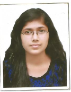
\includegraphics{Capture.PNG}
\end{center}
\end{figure}

\noindent\makebox[\linewidth]{\rule{\paperwidth}{0.4pt}}


\textbf{\underline{Address:}}
\hfill
\textbf{\underline{contact:}}\\
Wz- 528C/1 Sri Nagar, Rani Bagh, 
\hfill
9717288483
\\New Delhi-110034
\hfill
jindalshivani11@gmail.com
\section{Career Objective}
My main aim is to develop good applications, I want to be an \textbf{android app developer}.
\section{Education}
\begin{tabular}{||l | l | l | l | l||}
\hline
Deg/Sem & Institute & University/Board & Passing Year & Percentage/CGPA\\
\hline
Semester 2 & B.V.C.O.E & G.G.S.I.P.U & 2018 & 8.67 \\
\hline
Semester 1 & B.V.C.O.E & G.G.S.I.P.U & 2018 & 8.963\\
\hline
12$^{th}$ Board & KIIT WORLD SCHOOL & CBSE & 2016 & 83.4\%\\
\hline
10$^{th}$ Board & V.B.P.S & CBSE & 2014 & 9.2\\
\hline
\end{tabular}

\section{Projects}
\begin{enumerate}
\item \href{https://github.com/jindalshiva/heart}{ An android app that will help you to improve your health issues}
\item \href{https://github.com/jindalshiva/GooglePlacesGoogleMaps} { Google map app}
\item \href{https://github.com/jindalshiva/ISTY_1.2.3-master-master} { home automation}

\end{enumerate}
\end{document}
